\newcommand{\homedir}{/home/bscholtz/workspace-latex/templates/BasicTemplateUCT/}

%######################Preamble######################
\input{"\homedir preamble.tex"}

\newcommand{\coursecode}{EEE4036A}
\newcommand{\assignment}{Design Project (Team 14)}
\newcommand{\lecturer}{Riana Geschke}

\pagestyle{fancy}
\fancyhf{}
\rhead{Design Project}
\lhead{Team 14}
\cfoot{\thepage}

\begin{document}

%######################Title Page######################
\begin{titlepage} 

\includegraphics[width = 17cm]{images/uctbanner.png} \\

\begin{center}
\begin{LARGE}
Faculty of Engineering and the Built Environment \\
Department of Electrical Engineering \\
\end{LARGE}
\end{center}

\begin{center}  
\begin{Huge}
\textbf{\coursecode}\\
\bigskip
\bigskip
\hrule
\assignment \\
\end{Huge}

\vspace*{\fill}

\hrule
\begin{center}
\textbf{Benjamin Scholtz (SCHBEN011)\\
Jarushen Govender (GVNJAR002)\\
Isaac Lebogang Khobo (KHBISA001)\\
Nasko Stavrev (STVATA001)\\}
4$^{th}$ year BSc. (Eng.) Electrical Engineering Department\\
Lecturer: \lecturer \\
\today
\end{center}
\bigskip
\hrule

\end{center}
\end{titlepage}

%######################Contents######################

\newpage
%\section*{Contents}
%\addcontentsline{toc}{section}{Contents}  
\tableofcontents

%######################Plagiarism Dec.######################
\newpage
\section*{Plagiarism Declaration}
\addcontentsline{toc}{section}{Plagiarism Declaration}
\textbf{DECLARATION:}
\begin{enumerate}
\item I know that plagiarism is wrong. Plagiarism is to use another’s work and to pretend that it is one’s own.
\item I have not allowed, and will not allow, anyone to copy my work with the intention of passing it off as his or her own work.
\item This assignment is my own work. I have not used the material in this assignment in any of my other assignments.
\item I have included internet article, book, or other material references used for this assignment.
\end{enumerate}

\textbf{Signed:} Benjamin Scholtz (SCHBEN011), Jarushen Govender (GVNJAR002), Isaac Lebogang Khobo (KHBISA001), Nasko Stavrev (STVATA001)\\
\hrule
\textbf{Date:} \today \\
\hrule

%######################Begin Content######################
\newcommand{\lsec}[1]{\normalsize{\textbf{#1}}\\}

\newpage

\section{TASK CLARIFICATION}
\subsection{Background}
UCT Upper campus has a number of parking areas for staff, students and visitors using cars to travel to campus. There are red, yellow, blue and unmarked bays on campus. In addition there are disabled and 
visitor parking bays on campus. These categories are assigned the highest priority. 

For every user, a parking category is assigned, and an associated annual fee is charged.  The purchase of a parking disk allows the staff member/student/visitor to search for a parking spot in the designated category on campus, but it is not guaranteed that one will be available, since parking bays are oversold. When arriving on campus, a driver of a car may spend some time searching for an available spot in the required category. Parking disks are generally linked to a person and only valid for the specific vehicle for which the disk has been purchased, except for student lift clubs.

The Traffic  Department  on  Upper  Campus  administrates  and  manages  all  aspects  related  to  parking  of vehicles.\cite{assignment}
 
\subsection{Problem Statement}
For  a  driver  entering  Upper  Campus  in  a  car,  it  is  not immediately  apparent  where  there  are  parking bays available.  This is a particular problem during peak times when a large number of cars arrive on campus, looking for parking at the same time. The design assignment is to solve this problem using the electrical engineering skills of each of the team members in your group.\cite{assignment}

The design assignment is:

\begin{itemize}
\item To provide information in an easily accessible format, to each driver of a car immediately on arrival on campus, on where all the vacant parking bays on campus are. This must be for the specific category of parking for this user.

\item To determine whether a vehicle is parked on a bay not designated for this user, for example a yellow disk holder parks on a red bay, or a visitor parks on a disabled parking bay, and make this available to the traffic department in real time.

\item To  allow electronic reconfiguration  of  traffic  bay allocations  on  special  occasions, for example during the summer school period, when there are many visitors requiring parking on campus.

\item To monitor and log the use of parking bays and the percentage of occupation of each parking area and make this available to the traffic department, for the purpose of planning.\cite{assignment}
\end{itemize}

\newpage
\section{CONTEXT OF DESIGN}
\subsection{Macroeconomic Factors}
STEEPLE.
\subsection{Microeconomic Factors}


\newpage
\section{DESIGN SPECIFICATION}
\subsection{Scope}
This specification covers the analysis, design, production timeline and considerations, and lifecycle of the upgraded UCT parking system. The specification is for a parking system on upper campus to be used primarily in allocated parking zones rather than dispersed parking bays. The parking system specifications aim to meet the requirements introduced in the client problem statement.

\subsection{Applicable Documents}
The following documents are applicable to the project and are of importance to the ultimate specifications of the project:
\begin{itemize}
\item Group Allocation
\item Group Project Assignment
\item Design Notes
\end{itemize}

\subsection{Characteristics}
\subsubsection{Functional Characteristics}
\lsec{Function 1: User interface} 
Information must be available in an easily accessible format to indicate to drivers where legal parking bays are located.
\lsec{Function 2} 
\lsec{Interface Characteristics} 
\subsubsection{Quality Assurance}
\lsec{Standards and Codes}
The design must meet the following standards and codes:
\begin{itemize}
\item IEEE Standards.
\item SABS Standards.
\item ICASA RF Regulations.
\item RF PCB Design Standards.
\end{itemize}

\lsec{Methods of Testing}
The design should be tested using the following method:
\begin{enumerate}
\item Periodic random parking bay testing.
\item HIL system testing.
\item Brute force user and operator interface testing.
\item Long term power system testing.
\item RF propagation testing.
\end{enumerate}

\lsec{Reliability Issues}

\subsubsection{Timescale}
\lsec{Design Schedule}
The embodiment design should be completed within the given period of just under two months, in time for hand in after the first UCT term.

\lsec{Development Schedule}
Thereafter the final design should be developed and tested within a period of 4 months; and certified with the relevant organisations within a period of 2 months.

\lsec{Production Schedule}
The final design should be prototyped over a period of 1 month and then any necessary changes completed within 1 month thereafter - a final product will be sent for production over the course of 1 month. The necessary traffic department staff training and student/user familiarisation will be completed during the production time period over a period of 2 months.

\lsec{Delivery Schedule}
The complete system will be installed and in use over the period of 1 month. 

\subsubsection{Economic Factors}
\lsec{Market Analysis}
\lsec{Design Costs}
\lsec{Development, Manufacturing, Distribution Costs}
\subsubsection{Ergonomic Factors}
\lsec{User needs}
\lsec{Ergonomics}
\lsec{Controls}
\subsubsection{Life-cycle}
\lsec{Distribution}
\lsec{Operation}
\lsec{Maintenance}
\lsec{Disposal}
\subsection{Acceptance Test Requirements}
\lsec{Function Test Requirements}
Test methods: Could be by inspection, theoretical modelling, simulation, laboratory functional demonstration, field trials, in-service measurements, etc.

\newpage
\section{CONCEPTUAL DESIGN}
\subsection{Design One}
Design One (D1) uses a triangulation system to locate the registered vehicle within the parking area. Each registered vehicle has a tag with a unique ID - this ID has the user data linked to it in a database on the server back-end. The location of each parking space is known, and with the knowledge of where the vehicle is located it can be determined whether the vehicle is legally parked or not. 
  
\subsubsection{System Diagram}
\subsubsection{System Components}
\lsec{Tags and Beacons}
Due to a triangulation system being used, in every parking area there are at least three beacons - with four being used to try to eliminate signal propagation issues. The tags and beacons make use of a Decawave DW1000 ultra-wideband transceiver chip that is controlled via SPI from a Atmel micro-controller. 

The master beacon sends a signal out to synchronise all the beacons to the same time reference. Each tag sends a signal periodically with the unique user ID, transmit time and battery level which is received by each of the beacons. The beacons all relay time of flight data back to the master beacon which performs a time difference of arrival (TDOA) calculation to determine where the tag is located.\cite{decawave-presentation}

The tags transmit with a period of 5-10 minutes. This reduces power consumption and signal noise level interference with other tags. The tags do not receive data. The tags will be accurate to within 10cm giving more than enough accuracy for the application. The initial conservative battery life estimate is 5 years with proper power management in software. They will be powered with a LiPo battery that will need to be replaced or charged when discharged.

The beacons will use the same circuitry, but with different software running on the Atmel micro-controller. They will be required to both transmit and receive. The beacons will be mounted on poles (both light and installed) distributed across the UCT campus - this will allow the location of vehicles in any area. They will be powered with LiPo batteries which will be charged with solar panels - or wired in cases where this is not practical.

\lsec{Server Back-end}
The server back-end connects with the master beacon via WiFi and receives the tag location, unique ID and battery level for every new vehicle. This is updated on a database every 5-10 minutes. Further calculations and visualizations are performed and stored in the database to send to the end user. The following data will be available for each unique ID:

\begin{itemize}
\item User privileges.
\item Tag location (updated periodically).
\item Tag battery level (updated periodically).
\end{itemize}

\lsec{User Interface}
The user interface will connect with the server back-end to access the database and will relay the following data to the end user via a smart phone application or web application: 
\begin{itemize}
\item Indication of privilege level and violations.
\item Tag battery level.
\item Vehicle location.
\item Location of open parking bays.
\item Recommended parking area.
\item Number of free parking bays in parking area.
\item Traffic heat-map on campus.
\end{itemize}

\subsubsection{Requirement Satisfaction}

\subsubsection{Evaluation}
\lsec{Cost} 
(implementation, maintenance, energy consumption) \\
\lsec{Strong/weak Points}

\subsubsection{Risk Assessment}
\lsec{External Causes} 
(weather, vehicle impact, human interference) \\
\lsec{Intended Life}
risk of failure during intended life \\
\lsec{Mitigation}
mitigation (steps you will take to reduce the risk) \\

\subsection{Design Two}
\subsubsection{System Diagram}
\subsubsection{System Components}
\subsubsection{Requirement Satisfaction}

\subsubsection{Evaluation}
\lsec{Cost} 
(implementation, maintenance, energy consumption) \\
\lsec{Strong/weak Points}

\subsubsection{Risk Assessment}
\lsec{External Causes} 
(weather, vehicle impact, human interference) \\
\lsec{Intended Life}
risk of failure during intended life \\
\lsec{Mitigation}
mitigation (steps you will take to reduce the risk) \\

\newpage
\subsection{Weighted Selection}
The following weighted selection tables were formed and weights given to each aspect of the system design in order to determine which design meets the requirements outlined in the design specification:

\begin{table}[H]
\centering
\caption{Weighted selection: Design One\cite{handout}}
\label{my-label}
\begin{tabular}{l|l|l|l|}
\textbf{Aspect}                      & \textbf{Score (1-5)} & \textbf{Weight} & \textbf{Total} \\ \hline
Functionality / User satisfaction    & 5                     & 20                & 20               \\
Cost of implementation / Maintenance & 5                     & 40                & 40               \\
Reliability / Safety                 & 4                     & 10                & 8                \\
Ease of installation / Maintenance   & 5                     & 20                & 20               \\
Life span                            & 3                     & 10                & 6                \\ \hline
\textbf{Total score (100):}          &                       &                   & 94              
\end{tabular}
\end{table}

\begin{table}[H]
\centering
\caption{Weighted selection: Design Two\cite{handout}}
\label{my-label}
\begin{tabular}{l|l|l|l|}
\textbf{Aspect}                      & \textbf{Score (1-5)} & \textbf{Weight} & \textbf{Total} \\ \hline
Functionality / User satisfaction    & 3                     & 20                & 12               \\
Cost of implementation / Maintenance & 3                     & 40                & 24               \\
Reliability / Safety                 & 4                     & 10                & 8                \\
Ease of installation / Maintenance   & 4                     & 20                & 16               \\
Life span                            & 4                     & 10                & 8                \\ \hline
\textbf{Total score (100):}          &                       &                   & 68              
\end{tabular}
\end{table}

\subsection{Recommendation}
Based on the weighted selection and evaluation above, Design One should be further developed as a viable parking system solution for UCT upper campus. The embodiment design should be completed along with the necessary analysis and system testing.

\newpage
\section{EMBODIMENT DESIGN}
\subsection{System Overview}
\subsubsection{System Description}
\subsubsection{System Diagram}
\subsection{System Analysis}
Analysis of system operation, interfaces, use etc.
\subsection{Software Design}
\subsection{Mechanical Design} 
\subsubsection{Mechanical Requirements}
Durability, forces, dynamics.
\subsubsection{Technical Drawings}
\subsection{Electrical Design} 
\subsubsection{Power Requirements}
Battery life etc.
\subsubsection{Schematics}

\begin{figure}[H]
\begin{center}
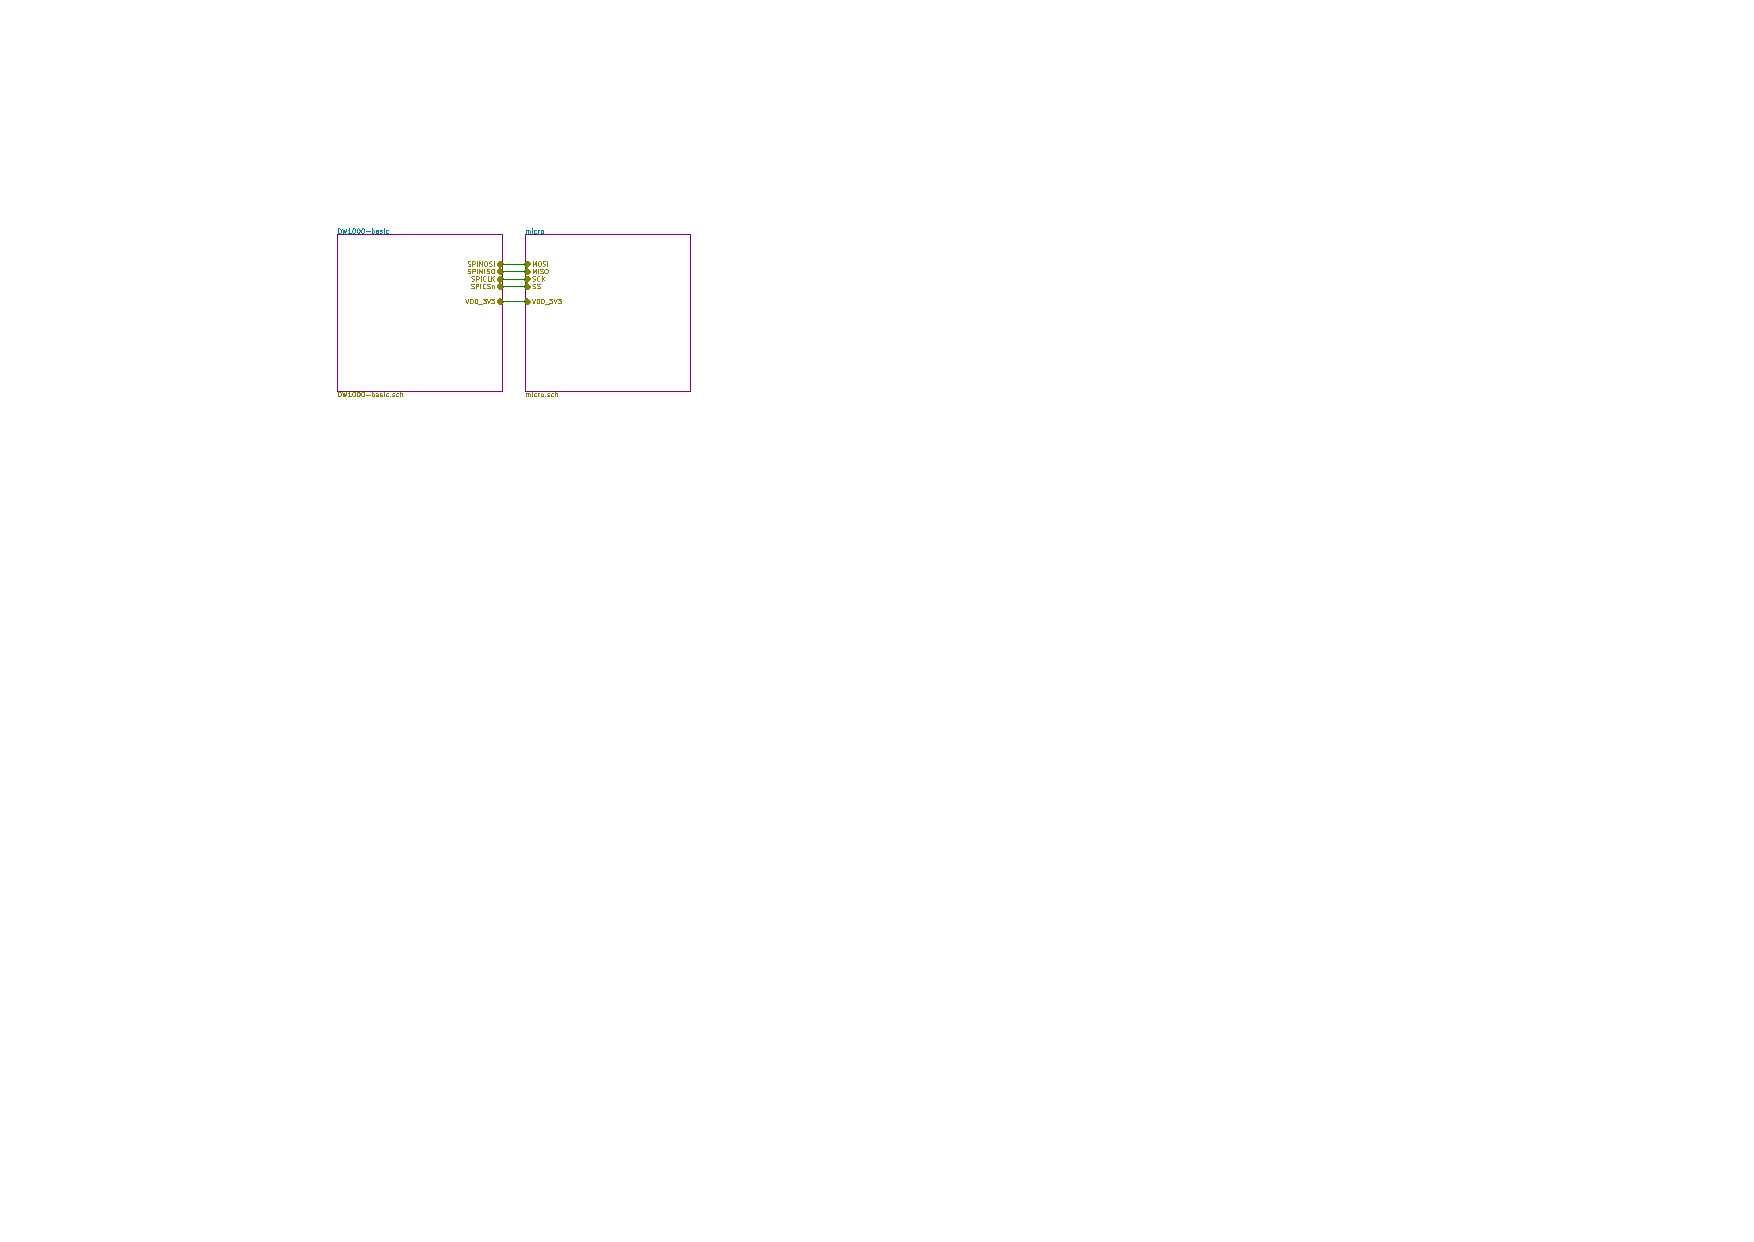
\includegraphics[page=1,scale=2,trim={5cm 14cm 17cm 3cm},clip]{data/parking-system.pdf}
\caption{Parking system tag schematic diagram: interface connections.}
\end{center}
\end{figure}

\begin{figure}[H]
\begin{center}
\includegraphics[page=2,scale=0.5,trim={0cm 0cm 0cm 0cm},clip]{data/parking-system.pdf}
\caption{Parking system tag schematic diagram: transceiver chip.}
\end{center}
\end{figure}

\begin{figure}[H]
\begin{center}
\includegraphics[page=3,scale=1,trim={10cm 8cm 10cm 5cm},clip]{data/parking-system.pdf}
\caption{Parking system tag schematic diagram: micro-controller.}
\end{center}
\end{figure}

\subsubsection{PCB Design}

\begin{figure}[H]
\begin{center}
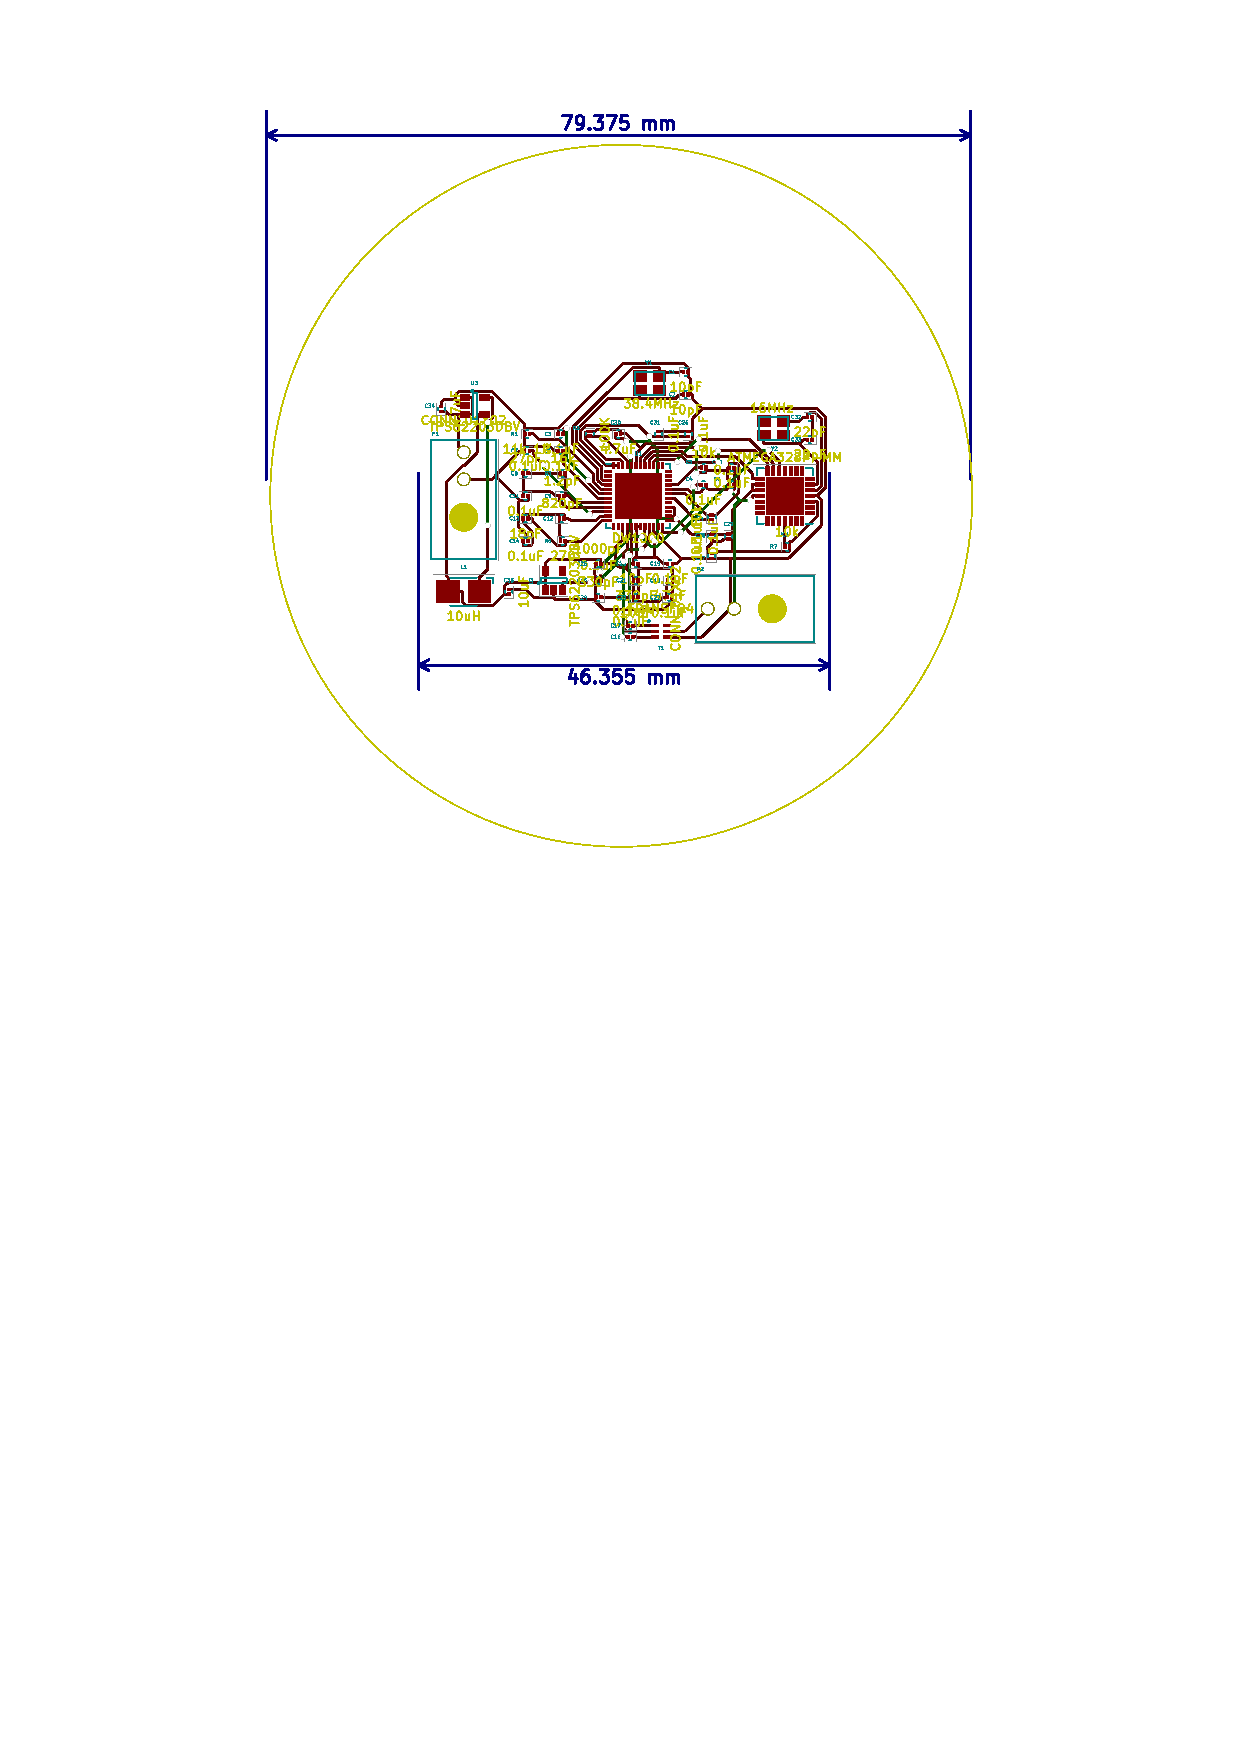
\includegraphics[trim={4cm 15cm 4cm 1cm},clip]{data/pcb-layout.pdf}
\caption{Parking system tag PCB layout.}
\end{center}
\end{figure}

\subsection{Assumptions}
Identify and show that checked validity.
\subsection{Failure Modes}
Probabilities,Consequences,Mitigation
\subsection{System Lifetime}
A statement of the design life time, with explanation of what (if anything) will limit it.
\subsection{Worst Case Calculation}
For at least one component / sub-system 

%\begin{figure}[H]
%\begin{center}
%\includegraphics[trim={Lcm Bcm Rcm Tcm},clip]{images/Fig1.pdf}
%\caption{•}
%\end{center}
%\end{figure}

%\begin{minted}[linenos=true]{matlab}
%\end{minted}

%######################References######################
\newpage
%\input{"\homedir references.tex"} %manual references

\bibliography{bibliography}
\bibliographystyle{ieeetran}
\addcontentsline{toc}{section}{References}


%######################Appendices######################
\newpage
\section*{Appendices}
\subsection*{Appendix A: Contributions}
\addcontentsline{toc}{section}{Appendix A: Contributions}
\subsection*{Appendix B: Progress Reports}
\addcontentsline{toc}{section}{Appendix B: Progress Reports}

\end{document}

%----------------------------------------------------------------------------


